\documentclass[conference]{IEEEtran}

\usepackage{cite}
\usepackage{amsmath,amssymb,amsthm}
\usepackage{graphicx}
\usepackage{booktabs}
\usepackage{array}
\usepackage{multirow}
\usepackage{url}
\usepackage[hidelinks,hypertexnames=false]{hyperref}
\usepackage{algorithm}
\usepackage{algpseudocode}
\usepackage{xcolor}
\usepackage{tikz}
\usetikzlibrary{arrows.meta,positioning,fit,calc}

\newcolumntype{L}[1]{>{\raggedright\arraybackslash}p{#1}}
\theoremstyle{definition}
\newtheorem{definition}{Definition}

\begin{document}

\title{Read Before You Run: Zero-Execution Detection of Malicious Agent Skills}

\author{\IEEEauthorblockN{Anonymous Submission}}
\hypersetup{
  pdftitle={Read Before You Run: Zero-Execution Detection of Malicious Agent Skills},
  pdfauthor={}
}

\maketitle

\begin{abstract}
Agent Skills combine persistent natural-language instructions with code,
configuration, and resources, allowing an untrusted package to shape an
agent's reasoning while inheriting its access to files, credentials, networks,
and processes. We study whether malicious Skills can be filtered before any
target content is installed, imported, or executed. \emph{Read Before You Run}
extracts bounded high-level descriptions, instruction semantics, normalized
sensitive operations, and cross-file Python call and taint paths; a
schema-constrained reviewer returns \textsc{Pass}, \textsc{Review}, or
\textsc{Block} with source-grounded evidence and explicit unknowns. On a
1,000-package source-disjoint benchmark, however, the complete method reaches
only 57/491 (11.61\%) malicious recall and 20.77\% F1 on 977 common successful
samples. Its 1/486 (0.21\%) false-positive rate is low, but a one-call document
baseline attains 36.15\% F1 and significantly more correct predictions
($p=3.17\times10^{-12}$). Removing the independently extracted high-level
function also does not hurt detection. The static front end nevertheless scans
1,000 current community Skills without failure, producing auditable candidates
without executing them. These results delimit, rather than overstate, the
current capability of zero-execution Skill screening: structured evidence
supports low-FPR triage and inspection, but does not yet improve source-disjoint
detection over direct semantic review.
\end{abstract}

\section{Introduction}
\label{sec:introduction}

Agent Skills turn instructions into supply-chain artifacts. A Skill can bundle
persistent natural-language directives with scripts, manifests, installation
commands, and external resources. Once admitted, this package influences an
agent while inheriting its access to files, credentials, networks, and
processes. The first security decision is therefore not whether a particular
action should run, but whether the package should enter the agent's trust
boundary at all.

The threat is already visible in public ecosystems. A recent measurement of
98,380 Skills confirmed 157 malicious packages through static triage, sandbox
execution, and expert review~\cite{liu2026maliciousskills}. This workflow
produces strong behavioral evidence, but only after a candidate is executed and
its trigger is reached. Runtime defenses likewise mediate an agent after
admission. Registries, enterprise gateways, and local agents still need a
pre-installation filter that can inspect untrusted packages without invoking
their code or dependencies.

That constraint makes the problem fundamentally ambiguous. Sensitive file
access, network transfer, process creation, and credential use are both useful
automation primitives and components of collection, exfiltration, or remote
execution. Instructions may state intent, conceal it, or redefine the apparent
purpose of the package. Static paths connect operations across files, yet a
connected path alone does not establish authorization. Existing Skill
detectors recover increasingly rich artifact evidence~\cite{wang2026malskills},
but recent source-disjoint evaluation shows that repository provenance can
dominate apparent accuracy~\cite{wang2026maliciousskillbench}. The unresolved
question is therefore empirical: \emph{does structured, source-grounded static
evidence improve malicious-Skill detection beyond direct semantic review when
provenance is separated?}

We answer this question with \emph{Read Before You Run}, a zero-execution
analysis pipeline. The detector reads every target file as bounded data and
keeps the package's boundary description separate from operational
instructions and implementation. It normalizes sensitive objects and
operations, constructs cross-file Python call graphs with fixed-point
interprocedural taint summaries, and preserves unresolved calls, unsupported
languages, truncation, and invalid outputs. A schema-constrained reviewer can
therefore return \textsc{Pass}, \textsc{Review}, or \textsc{Block} while citing
the evidence used for each finding.

The source-disjoint experiment rejects the hoped-for accuracy advantage. On
the 977 packages successfully processed by all compared methods, Ours produces
one false positive but detects only 57/491 malicious Skills. A one-call model
that sees only the primary Skill document detects 109/491 at comparable
precision and is significantly more accurate. The independently extracted
high-level function also provides no measurable benefit on the smaller
benchmark. In contrast, the same pipeline appears strong on a 200-package set
whose labels are perfectly confounded with provenance. The comparison exposes
a practical boundary: structured evidence supports low-false-positive triage
and auditable inspection, but does not yet improve source-disjoint detection
over direct document review.

This paper makes three contributions:
\begin{itemize}
  \item \textbf{A traceable zero-execution pipeline} that connects constrained
  instruction analysis, versioned sensitive-object rules, cross-file call
  recovery, and interprocedural taint summaries without loading target code.
  \item \textbf{A source-disjoint comparison} against frozen rules and direct
  document classification, reporting paired significance, processing failures,
  model cost, and three-way review workload rather than accuracy alone.
  \item \textbf{A falsification result for structured Skill detection:} the
  complete pipeline and its high-level function view fail to improve detection
  over direct semantic review, while retaining a low-FPR, evidence-bearing
  operating point and scalable audit front end.
\end{itemize}

Section~\ref{sec:background} defines the threat model,
Section~\ref{sec:related} reviews adjacent defenses,
Section~\ref{sec:methodology} presents the detector, and
Section~\ref{sec:evaluation} evaluates its supported and rejected claims.

\section{Background and Threat Model}
\label{sec:background}

\subsection{Agent Skill Packages}

An Agent Skill is treated as a versioned package containing a primary skill
document and any referenced instructions, scripts, configuration, manifests,
and resources.  The package boundary is the unit of analysis.  A single
document may mix user-facing descriptions with operative instructions, so
content roles are assigned at section or paragraph granularity rather than by
filename alone.

\subsection{Threat Model}

The adversary controls every untrusted byte in the package and may distribute
behavior across artifacts.  The adversary knows the analysis strategy and may
use paraphrase, aliases, indirection, string construction, dynamic imports,
reflection, simple encoding, or opaque binaries.  The detector and its policy
and rule versions are trusted.  The detector neither installs dependencies nor
imports, invokes, or executes target-supplied content, and it does not contact
endpoints named by the package.

The method does not claim to recover code obtained only at runtime, behavior
inside unavailable dependencies, or semantics hidden in unrecoverable encrypted
or binary content.  Such uncertainty is represented in the output.  In
particular, \textsc{Pass} is not a proof of safety.

\subsection{Design Goals}

The detector should (G1) remain zero execution; (G2) preserve independence
between high-level function and internal behavior; (G3) connect cross-file
evidence; (G4) reduce false positives on legitimate sensitive operations;
(G5) expose uncertainty instead of silently treating missing analysis as
benign; and (G6) return evidence that a reviewer can locate in the original
package.

\section{Related Work}
\label{sec:related}

\subsection{Agent Skills as a Supply-Chain Boundary}

Agent Skills occupy an unusual point between prompts and packages: they combine
natural-language control with executable code, configuration, and resources.
Liu et al. establish the ecosystem threat through a large-scale measurement of
public registries, using static candidate generation followed by sandbox
execution and expert confirmation~\cite{liu2026maliciousskills}. MalSkills
instead targets zero-execution detection by extracting security-sensitive
operations, linking values across artifacts, and applying neuro-symbolic rules
to a dependency graph~\cite{wang2026malskills}. MaliciousSkillBench consolidates
multiple Skill sources and demonstrates that performance degrades when the
evaluation separates provenance~\cite{wang2026maliciousskillbench}. Together,
these works define the central tension for admission control: behavioral
confirmation requires execution, whereas artifact-only detection must reason
under ambiguity and distribution shift.

The broader software-supply-chain literature exposes a complementary entry
point. Code-generating models frequently hallucinate plausible package names,
creating opportunities for package-confusion attacks~\cite{spracklen2025package}.
That work asks which dependency an LLM causes a developer to select; malicious
Skill detection asks what an already selected package can instruct and enable
an agent to do. Our work is closest to MalSkills, but evaluates whether adding
separated high-level context to recovered behavior improves detection under a
source-disjoint protocol. The result is negative, delimiting this design point
rather than treating richer structure as an assumed benefit.

\subsection{Adversarial Instructions, Tools, and Agent State}

Prompt injection studies an attacker who places competing instructions in
content consumed by an application. Liu et al. formalize this problem and
benchmark attacks and defenses across models and tasks
~\cite{liu2024promptinjection}. InjecAgent specializes the threat to
tool-integrated agents, covering harmful actions and private-data exfiltration
triggered by tool-returned content~\cite{zhan2024injecagent}. These attacks occur
during a task trajectory, whereas a malicious Skill can make adversarial
instructions persistent and package them with helper code or installation
behavior.

Other work compromises different components of the agent stack. AgentPoison
plants retrieval triggers in long-term memory or knowledge bases
~\cite{chen2024agentpoison}; BadAgent inserts backdoors through an untrusted
model or fine-tuning data~\cite{wang2024badagent}. ToolSword maps failures across
tool-use input, execution, and output stages~\cite{ye2024toolsword}, while
ToolAlign trains for helpful, harmless, and autonomous tool use
~\cite{chen2024toolalign}. These studies show that agent behavior can be
subverted through model weights, memory, retrieved content, or tool feedback.
Our adversary instead controls a distributable Skill artifact. The detector
therefore cannot retrain the underlying model or observe a trigger at runtime;
it must identify suspicious instructions and implementation evidence before
the artifact becomes agent state.

\subsection{Dynamic Analysis and Agent Security Evaluation}

Dynamic approaches judge security from execution trajectories. AgentFuzz uses
directed greybox fuzzing, generated seeds, and semantic and distance feedback
to trigger taint-style vulnerabilities in running agent applications
~\cite{liu2025agentfuzz}. ToolEmu searches for long-tail failures in
language-model-emulated tool environments without invoking real services
~\cite{ruan2024toolemu}. AgentDojo combines utility tasks, security goals, and
indirect prompt-injection attacks in a reproducible agent environment
~\cite{debenedetti2024agentdojo}; Agent Security Bench spans prompt, memory,
tool, and multi-agent attack surfaces~\cite{zhang2025asb}.

These evaluations observe whether an agent performs a prohibited action, which
provides a semantically direct outcome but depends on an executable system and
a triggering interaction. Static package analysis moves the decision earlier:
it can cover dormant artifacts without running them, but must expose uncertain
reachability, unsupported languages, and incomplete parsing. Our evaluation
therefore reports class-conditional detection together with processing
coverage, abstention, and unresolved outputs. It does not treat the absence of
a recovered static path as evidence that no runtime behavior exists.

\subsection{Instruction Integrity and Runtime Enforcement}

Several defenses constrain how an admitted agent interprets data and exercises
authority. StruQ separates instructions from data through a structured query
interface and model training~\cite{chen2025struq}. Task Shield checks whether
candidate instructions and tool calls advance the user's declared objective
~\cite{jia2025taskshield}. CaMeL derives control flow from trusted input and
tracks capabilities on values passed to tools~\cite{debenedetti2026camel}.
These mechanisms target indirect injection during task execution; they can
mediate actions even when the underlying package is already present.

System mechanisms enforce the same principle below the prompt layer.
IsolateGPT places third-party agent applications in separate contexts with
explicit interfaces~\cite{wu2025isolategpt}, while AgentSpec provides a policy
language for runtime constraints over agent actions~\cite{wang2026agentspec}.
Isolation and policy enforcement limit consequences but do not decide whether
an artifact is trustworthy before installation. Conversely, a static
admission decision cannot observe environment-dependent behavior and cannot
replace least privilege after admission. Read Before You Run occupies this
upstream boundary: it produces source-grounded pass/review/block evidence for
the package, leaving runtime mediation to complementary defenses.

\section{Methodology}
\label{sec:methodology}

\subsection{Overview}

Let $S$ be one immutable Skill package containing instructions, source code,
configuration, and auxiliary files.  The detector computes
\begin{equation}
\mathcal{A}(S)=(z,F,U,\Gamma), \qquad
z\in\{\textsc{Pass},\textsc{Review},\textsc{Block}\},
\label{eq:detector}
\end{equation}
where $F$ contains source-grounded findings, $U$ records unresolved analysis,
and $\Gamma$ records coverage. Equation~\ref{eq:detector} defines the complete
detector output. The package is never imported, installed, or
executed.  Figure~\ref{fig:method} gives the pipeline.  It constructs two
independent views: a high-level summary of what the Skill presents at its
boundary, and a static account of what its instructions and implementation can
do.  The views meet only during security review.

\begin{figure*}[!t]
  \centering
  \resizebox{0.98\textwidth}{!}{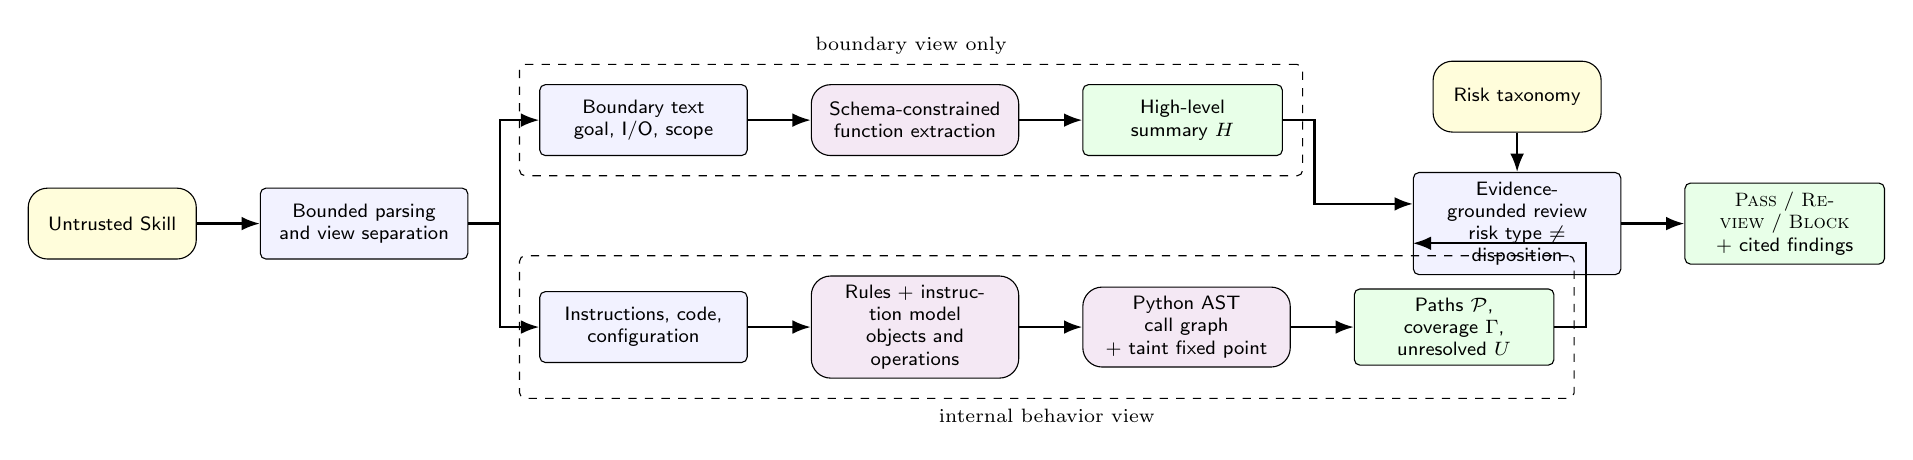
\begin{tikzpicture}[
  font=\sffamily\scriptsize, >=Latex, node distance=5mm and 8mm,
  box/.style={draw, rounded corners=2pt, minimum height=9mm, text width=24mm, align=center, fill=blue!5},
  data/.style={draw, rounded corners=7pt, minimum height=9mm, text width=19mm, align=center, fill=yellow!14},
  process/.style={draw, rounded corners=7pt, minimum height=9mm, text width=24mm, align=center, fill=violet!9},
  output/.style={draw, rounded corners=2pt, minimum height=9mm, text width=23mm, align=center, fill=green!9},
  arrow/.style={->, thick}
]
\node[data] (skill) {Untrusted Skill};
\node[box, right=of skill] (parse) {Bounded parsing\\and view separation};
\node[box, above right=4mm and 9mm of parse] (boundary) {Boundary text\\goal, I/O, scope};
\node[process, right=of boundary] (summary) {Schema-constrained\\function extraction};
\node[output, right=of summary] (h) {High-level summary $H$};
\node[box, below right=4mm and 9mm of parse] (artifacts) {Instructions, code,\\configuration};
\node[process, right=of artifacts] (extract) {Rules + instruction model\\objects and operations};
\node[process, right=of extract] (graph) {Python AST call graph\\+ taint fixed point};
\node[output, right=of graph] (paths) {Paths $\mathcal{P}$, coverage $\Gamma$,\\unresolved $U$};
\node[box, right=12mm of $(h)!0.5!(paths)$] (review) {Evidence-grounded review\\risk type $\neq$ disposition};
\node[output, right=of review] (verdict) {\textsc{Pass} / \textsc{Review} / \textsc{Block}\\+ cited findings};
\node[data, above=of review] (taxonomy) {Risk taxonomy};
\draw[arrow] (skill) -- (parse);
\draw[arrow] (parse.east) -- ++(4mm,0) |- (boundary.west);
\draw[arrow] (parse.east) -- ++(4mm,0) |- (artifacts.west);
\draw[arrow] (boundary) -- (summary); \draw[arrow] (summary) -- (h);
\draw[arrow] (artifacts) -- (extract); \draw[arrow] (extract) -- (graph); \draw[arrow] (graph) -- (paths);
\draw[arrow] (h.east) -- ++(4mm,0) |- ([yshift=2.5mm]review.west);
\draw[arrow] (paths.east) -- ++(4mm,0) |- ([yshift=-2.5mm]review.west);
\draw[arrow] (taxonomy) -- (review); \draw[arrow] (review) -- (verdict);
\node[draw,dashed,rounded corners=2pt,fit=(boundary)(summary)(h),inner sep=2.5mm,
      label={[font=\scriptsize]above:boundary view only}] {};
\node[draw,dashed,rounded corners=2pt,fit=(artifacts)(extract)(graph)(paths),inner sep=2.5mm,
      label={[font=\scriptsize]below:internal behavior view}] {};
\end{tikzpicture}
}
  \caption{Zero-execution analysis. Boundary text produces a high-level
  functional summary. Operative instructions, code, and configuration produce
  evidence records and a cross-file behavior graph. The final reviewer combines
  both views with the risk taxonomy and explicit coverage.}
  \label{fig:method}
\end{figure*}

\subsection{Artifact Parsing and View Separation}
\label{sec:parsing}

\textbf{Input and bounds.} The parser accepts either a directory, regular
files streamed from a fixed Git commit, or one selected subtree of a repository
archive. It skips symbolic links and dependency/build directories and enforces
limits of 128 files, 256~KiB per file, and 750,000 decoded characters per
package. Archive members with absolute paths, parent traversal, or symbolic
link type are ignored. Reaching a bound sets a truncation flag; it does not
turn omitted content into benign evidence.

\textbf{Separated views.} The parser treats \texttt{SKILL.md} as a mixed
document. Name, description, overview, purpose, usage, inputs, outputs, and
capability sections form the boundary view $T_H$. Operational sections such
as instructions, setup, commands, rules, and examples form the instruction
view $T_I$. Fenced code is excluded from $T_H$. Every instruction paragraph
retains its file and first line. Source and configuration files form $T_C$
and $T_K$; neither is exposed to high-level extraction. Ambiguous prose is
excluded from $T_H$ rather than allowing implementation details to enlarge the
Skill's stated function.

\textbf{Output.} This stage emits $(T_H,T_I,T_C,T_K)$, a file inventory, and
initial coverage $\Gamma_0$. The two downstream branches receive disjoint
inputs.

\subsection{High-Level Function Extraction}
\label{sec:function}

The function branch receives only $T_H$ and produces
\begin{equation}
H=(g,I,O,Q,E,V,c_H),
\label{eq:function-summary}
\end{equation}
where $g$ is the stated goal; $I$ and $O$ are input and output classes; $Q$ is
the stated operation scope and resource set; $E$ lists named external
services; $V$ lists visible side effects; and
$c_H\in\{\mathsf{sufficient},\mathsf{partial},\mathsf{minimal}\}$ describes
completeness. A schema-constrained language model performs extraction, not
security classification. Equation~\ref{eq:function-summary} is the only
information passed from this branch to review. The model receives neither
code, rules, risk findings, nor
labels. Empty or vague descriptions therefore yield sparse fields rather than
inferred permissions. Local validation rejects missing fields, additional
fields, and values outside the closed schema.

This separation is essential: if code were allowed to define $H$, an
implementation could justify any behavior after the fact. Conversely, a
minimal $H$ is not evidence of malice. It limits what can be established as
in-scope and increases uncertainty at review time.

\subsection{Static Behavior Recovery}
\label{sec:behavior}

The behavior branch extracts only security-relevant facts. Ordinary local
computation is retained only when it propagates a sensitive value or reaches a
security-sensitive operation.

\subsubsection{Instruction Evidence}

Rules first identify explicit instruction override, concealment, confirmation
bypass, safeguard weakening, destructive actions, and download--execute
idioms. A second schema-constrained model analyzes location-preserving
instruction segments to capture paraphrases. Each record contains an action,
object, destination, authorization state, user visibility, condition, segment
identifier, and confidence. The model is asked to extract requested behavior,
not to classify the package. Outputs that cite a nonexistent segment or use an
out-of-taxonomy action are retried and then rejected.

\subsubsection{Objects and Operations}

A versioned object library maps observable aliases, paths, environment names,
and API signatures to normalized classes such as SSH keys, cloud credentials,
API tokens, browser authentication data, password stores, wallet secrets, and
private communications. Each match retains object class, sensitivity, match
type, file, line, and confidence. Separately, operation rules locate read,
enumeration, network transfer, process creation, dynamic evaluation,
download--execute, persistence, privilege change, and destructive operations.
An object mention alone is not a malicious finding; it becomes useful only
when connected to an operation or an explicit hostile instruction.

\subsubsection{Cross-File Behavior Graph}

For Python artifacts, we parse abstract syntax trees without importing target
modules. Let $\mathcal{F}$ be the set of module bodies and top-level functions.
The graph
\begin{equation}
G=(V,E),\quad V=V_A\cup V_F\cup V_P,\quad
E=E_{\mathrm{contains}}\cup E_{\mathrm{calls}},
\label{eq:graph}
\end{equation}
contains artifact nodes $V_A$, function nodes $V_F$, and recovered taint-path
evidence $V_P$. Equation~\ref{eq:graph} separates package containment from
resolved call edges. Import aliases and local module names resolve calls across
files. Unresolved calls remain in $U$.

Value flow is computed over the finite domain
$\mathcal{D}=2^{\mathcal{S}\cup\mathcal{P}}$, where $\mathcal{S}$ contains
normalized sensitive-source labels and $\mathcal{P}$ contains symbolic formal
parameters. An environment $\rho_f:x\mapsto\mathcal{D}$ maps variables in
function $f$ to may-taint sets. Assignments copy sets, container and string
operations take their union, known transformations preserve taint, and source
APIs add an element of $\mathcal{S}$. For each function we compute
\begin{equation}
\Sigma_f=(R_f,K_f,C_f),
\label{eq:summary}
\end{equation}
where $R_f$ is the taint set that may reach a return, $K_f$ is the set of sink
facts, and $C_f$ is the set of resolved callees. The summary in
Equation~\ref{eq:summary} is parameterized by symbolic formal inputs. At a call
$f\rightarrow g$,
formal labels in $\Sigma_g$ are substituted with the caller's argument sets;
returned labels and sink facts are then propagated into $f$. Call traces are
canonicalized as simple paths, so recursive cycles cannot grow summaries
indefinitely. Because transfer functions are monotone and $\mathcal{D}$ is
finite, repeated summary evaluation reaches a fixed point:
\begin{equation}
\Sigma^{(i+1)}=\mathcal{T}(\Sigma^{(i)}),\qquad
\Sigma^{*}=\mathcal{T}(\Sigma^{*}).
\label{eq:fixedpoint}
\end{equation}
Equation~\ref{eq:fixedpoint} terminates because the transfer is monotone over a
finite domain.

A reported path is
\begin{equation}
\pi=\langle s,f_0,f_1,\ldots,f_k,q,d,L\rangle,
\label{eq:behavior-path}
\end{equation}
where $s$ is a normalized sensitive source, $f_0\ldots f_k$ is the recovered
call chain, $q$ is a network or process sink, $d$ is its literal destination
when available, and $L$ contains source and sink locations. This distinguishes
a connected source-to-sink flow from two unrelated keyword matches;
Equation~\ref{eq:behavior-path} is the evidence record exposed to review.

\begin{figure}[!t]
  \centering
  \resizebox{0.98\columnwidth}{!}{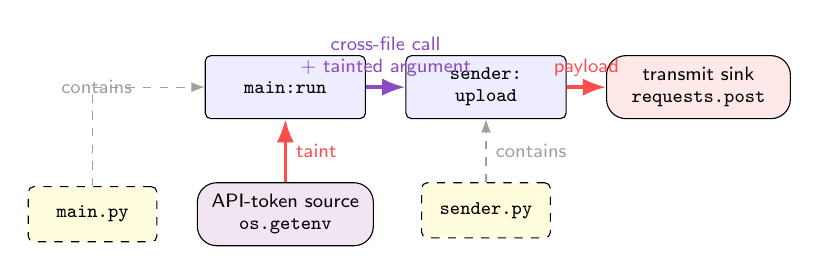
\begin{tikzpicture}[
  font=\sffamily\scriptsize, >=Latex, node distance=8mm and 5mm,
  artifact/.style={draw, dashed, rounded corners=2pt, fill=yellow!13,
    minimum height=7mm, text width=14mm, align=center},
  function/.style={draw, rounded corners=2pt, fill=blue!7,
    minimum height=8mm, text width=18mm, align=center},
  source/.style={draw, rounded corners=7pt, fill=violet!10,
    minimum height=8mm, text width=20mm, align=center},
  sink/.style={draw, rounded corners=7pt, fill=red!9,
    minimum height=8mm, text width=21mm, align=center},
  contains/.style={->, dashed, gray!75},
  callflow/.style={->, very thick, blue!65!red!70},
  flow/.style={->, very thick, red!70}
]
\node[function] (run) {\texttt{main:run}};
\node[function, right=of run] (upload) {\texttt{sender:}\\\texttt{upload}};
\node[sink, right=of upload] (post) {transmit sink\\\texttt{requests.post}};
\node[source, below=of run] (secret) {API-token source\\\texttt{os.getenv}};
\node[artifact, left=of secret] (main) {\texttt{main.py}};
\node[artifact, below=of upload] (sender) {\texttt{sender.py}};

\draw[contains] (main) |- node[pos=.72,left]{contains} (run);
\draw[contains] (sender) -- node[right]{contains} (upload);
\draw[flow] (secret) -- node[right]{taint} (run);
\draw[callflow] (run) -- node[above,align=center]{cross-file call\\+ tainted argument} (upload);
\draw[flow] (upload) -- node[above]{payload} (post);
\end{tikzpicture}
}
  \caption{Example cross-file path recovered by the implemented analyzer.
  Function summaries substitute the caller's API-token taint for the callee's
  formal parameter and propagate it to the network payload.}
  \label{fig:behavior-graph}
\end{figure}

Figure~\ref{fig:behavior-graph} illustrates how a caller's sensitive value is
substituted into a callee summary and propagated to a network sink.

The current frontend constructs these paths for Python. JavaScript,
TypeScript, and shell files still receive operation and object scanning but are
listed as unsupported for syntax-tree flow recovery. Python parse errors,
reflection, unresolved dynamic dispatch, and computed destinations are also
reported in $U$. For artifacts without a recovered data-flow path, a same-file
line-window association may be retained as lower-confidence evidence with
unknown reachability; it is never presented as an interprocedural path.
Failure to reach the fixed point within the bounded round schedule is likewise
recorded in $U$ rather than treated as absence of flow.

\textbf{Output.} The behavior branch emits instruction records $B_I$, rule
evidence $B_R$, paths $\mathcal{P}$, graph $G$, unresolved items $U$, and
coverage $\Gamma$ (parsed files, functions, call edges, paths, parse failures,
unsupported code, and unresolved calls).

\subsection{Evidence-Grounded Security Review}
\label{sec:review}

The final reviewer receives $(H,B_I,B_R,\mathcal{P},U,\Gamma)$ under a closed
schema. Risk type and disposition are separate. Risk type follows three
domains: malicious attack (instruction hijacking, information theft, resource
destruction or leakage, and unauthorized operation), design defect (sensitive
information protection, input handling, authentication/authorization, and
runtime environment), and legal risk (copyright, privacy, compliance,
certificate, and license). Disposition depends on severity, evidence
confidence, authorization, impact, static reachability, and coverage; a severe
design defect can therefore be blocked without being labeled an intentional
attack.

For a behavior record $b$, review compares four observable dimensions with
$H$:
\begin{equation}
\begin{aligned}
R(H,b)&=(R_a,R_o,R_d,R_e),\\
R_j&\in\{\mathsf{supported},\mathsf{unsupported},\mathsf{unknown}\}.
\end{aligned}
\label{eq:consistency}
\end{equation}
corresponding to action, object scope, destination, and side effect. Exact
matches and explicit policy violations in Equation~\ref{eq:consistency} are
supplied as deterministic evidence;
the model handles bounded semantic cases. Every risk finding must cite an
existing instruction, rule, object, or graph evidence identifier. Local
validation enforces the citation set, risk taxonomy, JSON schema, and the
invariant that a malicious label has at least one malicious-attack finding.
Invalid output is retried at most three times; persistent failure is logged and
the package is excluded from binary metrics rather than counted benign.

Let $B$ denote a supported high-impact risk that warrants rejection and $W$
denote a material risk or uncertainty that requires review. The decision is
\begin{equation}
z=\begin{cases}
\textsc{Block}, & B,\\
\textsc{Review}, & \neg B\land W,\\
\textsc{Pass}, & \text{otherwise}.
\end{cases}
\label{eq:decision}
\end{equation}
Equation~\ref{eq:decision} keeps disposition separate from risk type.
\textsc{Pass} is consequently a statement about analyzed evidence, not a proof
that the package is harmless. The returned record includes the binary label,
three-way disposition, confidence, cited findings, graph coverage, and $U$.

\subsection{Analysis Invariants}

The design enforces three invariants. \emph{View separation} prevents internal
implementation from expanding $H$. \emph{Evidence grounding} restricts every
risk claim to identifiers produced by static extraction. \emph{Uncertainty
preservation} exposes unsupported languages, parse failures, unresolved calls,
truncation, and persistent model failures instead of treating them as negative
evidence. These invariants do not make static analysis complete; they delimit
what the detector is allowed to claim without running a Skill.

\section{Evaluation}
\label{sec:evaluation}

We evaluate four questions: \textbf{RQ1} whether the detector generalizes to
source-disjoint Skills; \textbf{RQ2} whether structured static evidence helps
beyond rules or direct document classification; \textbf{RQ3} what behavior the
graph actually recovers; and \textbf{RQ4} whether the pipeline fails safely and
scales to a current, unlabeled corpus. \textbf{Ours} denotes the complete
pipeline in Section~\ref{sec:methodology}.

\subsection{Experimental Setup}

\subsubsection{Datasets}

\textbf{MalSkillsBench-200.} We retain a fixed snapshot of the public
100-malicious/100-benign benchmark released with
MalSkills~\cite{wang2026malskills}, only as a diagnostic set.
Its labels are completely confounded with source and owner: source alone
predicts all labels, and every one of its 78 owners is class-pure. Results on
this corpus therefore cannot establish source-independent generalization.

\textbf{MaliciousSkillBench-SD1000.} Our primary labeled evaluation samples
500 malicious and 500 benign Skills from the official source-disjoint test
split of MaliciousSkillBench~\cite{wang2026maliciousskillbench}. The sample is
balanced, integrity-checked, and preserves the released labels while excluding
label and source fields from detector input. It spans three held-out source
groups (428, 425, and 147 packages).

\textbf{Community-Skills-1000.} To test current-corpus operability, we collect
100 Skills from each of ten registry categories: data, design, development,
DevOps, documents, marketing, product, productivity, security, and testing.
Selection is deterministic, capped at five Skills per repository, and retains
only the bounded primary Skill document. This corpus has no security ground
truth; its outputs are audit candidates, not estimates of malicious prevalence.

\subsubsection{Compared Methods}

\emph{Frozen rules} applies the same instruction, object, filesystem, network,
process, concealment, privilege, persistence, and destructive-operation rules
used to generate evidence for Ours, with a fixed score threshold of five.
\emph{Direct model} sends only the bounded primary Skill document to one
schema-constrained reviewer; it receives no static findings, graph, source,
registry metadata, or label. \emph{No function view} removes the independent
high-level summary while leaving the remaining Ours pipeline unchanged.

\subsubsection{Protocol and Metrics}

Targets are streamed as data and are never installed, imported, or executed.
Each package is bounded to 128 files, 256~KiB per file, and 750,000 characters.
Model stages use \texttt{deepseek-v4-flash}, temperature zero, thinking
disabled, closed JSON schemas, and deterministic local validation. Predictions
and failures are checkpointed per sample; two bounded resume passes retry only
unresolved samples. We report coverage separately and never impute failures.

Malicious is the positive class. We report Precision, Recall, F1, FPR,
accuracy, balanced accuracy, MCC, and three-way disposition. Confidence
intervals use 1,000 class-stratified bootstrap replicates with seed 1337.
Paired comparisons use the intersection of successful samples and an exact
McNemar test.

\subsection{RQ1: Source-Disjoint Detection}

Table~\ref{tab:source-disjoint} changes the conclusion suggested by the small
benchmark. On the 977 packages shared by all methods, Ours nearly eliminates
false positives, but detects only 57/491 malicious Skills. Direct document
classification doubles recall while retaining high precision, and is correct
on 54 samples that Ours misses versus four in the opposite direction
($p=3.17\times10^{-12}$). Thus, structured evidence does not outperform a
strong direct model under source separation.

\begin{table*}[!t]
\centering
\caption{Source-disjoint results on 977 common successful packages. Counts
precede percentages; higher is better except FPR.}
\label{tab:source-disjoint}
\small
\resizebox{\textwidth}{!}{%
\begin{tabular}{lrrrrrrrr}
\toprule
Method & TP/FP/TN/FN & Precision & Recall & F1 & FPR & Accuracy & Bal. Acc. & MCC \\
\midrule
Frozen rules & 53/53/433/438 & 53/106 (50.00\%) & 53/491 (10.79\%) & 17.76\% & 53/486 (10.91\%) & 486/977 (49.74\%) & 49.94\% & $-0.002$ \\
\textbf{Ours} & \textbf{57/1/485/434} & \textbf{57/58 (98.28\%)} & \textbf{57/491 (11.61\%)} & \textbf{20.77\%} & \textbf{1/486 (0.21\%)} & \textbf{542/977 (55.48\%)} & \textbf{55.70\%} & \textbf{0.241} \\
Direct model & 109/3/483/382 & 109/112 (97.32\%) & 109/491 (22.20\%) & 36.15\% & 3/486 (0.62\%) & 592/977 (60.59\%) & 60.79\% & 0.339 \\
\bottomrule
\end{tabular}%
}
\end{table*}

Bootstrap intervals reinforce the gap: Ours reaches 11.61\% recall
[8.76\%, 14.66\%] and 20.77\% F1 [16.10\%, 25.44\%], whereas the direct model
reaches 22.20\% recall [18.74\%, 25.87\%] and 36.15\% F1 [31.40\%, 40.90\%].
The precision difference is negligible relative to the recall loss.

\noindent\textbf{Finding 1.} The source-disjoint experiment rejects an overall
detection advantage for Ours; its supported advantage is a 0.21\% FPR at the
cost of very low malicious recall.

\subsection{RQ2: What Produces the Decision?}

The source-confounded 200-package diagnostic explains why the earlier result
was misleading. Ours attains 54/55 (98.18\%) precision, 54/99 (54.55\%) recall,
and 70.13\% F1 on 197 completed packages, versus 32.47\% F1 for frozen rules.
That improvement disappears under source separation. Moreover, removing the
high-level function view slightly improves the 196-sample common subset from
70.13\% to 71.79\% F1; only two predictions change, both correcting false
negatives ($p=0.50$). The evidence therefore falsifies the intended
function--behavior consistency contribution on the available benchmark.

Ours' low binary FPR is achieved through abstention rather than benign
resolution. Figure~\ref{fig:triage} shows the source-disjoint common subset:
277/491 malicious packages are contained by \textsc{Block} or
\textsc{Review}, but 244/486 benign packages also require review. Only
241/486 benign Skills pass automatically.

\begin{figure}[!t]
  \centering
  \resizebox{0.98\columnwidth}{!}{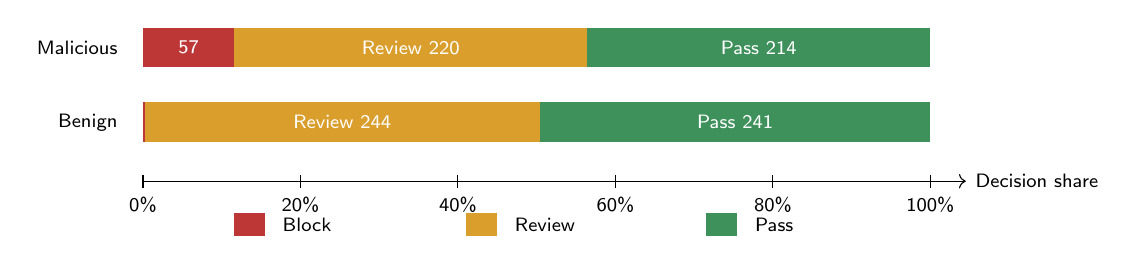
\begin{tikzpicture}[font=\sffamily\scriptsize]
  \definecolor{blockred}{RGB}{190,55,55}
  \definecolor{reviewgold}{RGB}{218,158,44}
  \definecolor{passgreen}{RGB}{63,145,92}
  \draw[->] (0,0) -- (10.45,0) node[right] {Decision share};
  \foreach \x/\lab in {0/0,2/20,4/40,6/60,8/80,10/100}
    \draw (\x,0.08) -- (\x,-0.08) node[below] {\lab\%};
  \node[anchor=east] at (-0.2,1.7) {Malicious};
  \fill[blockred] (0,1.45) rectangle (1.161,1.95);
  \fill[reviewgold] (1.161,1.45) rectangle (5.642,1.95);
  \fill[passgreen] (5.642,1.45) rectangle (10,1.95);
  \node[text=white] at (0.581,1.70) {57};
  \node[text=white] at (3.402,1.70) {Review 220};
  \node[text=white] at (7.821,1.70) {Pass 214};
  \node[anchor=east] at (-0.2,0.75) {Benign};
  \fill[blockred] (0,0.50) rectangle (0.021,1.00);
  \fill[reviewgold] (0.021,0.50) rectangle (5.041,1.00);
  \fill[passgreen] (5.041,0.50) rectangle (10,1.00);
  \node[text=white] at (2.531,0.75) {Review 244};
  \node[text=white] at (7.521,0.75) {Pass 241};
  \fill[blockred] (1.15,-0.70) rectangle (1.55,-0.40);
  \node[anchor=west] at (1.65,-0.55) {Block};
  \fill[reviewgold] (4.10,-0.70) rectangle (4.50,-0.40);
  \node[anchor=west] at (4.60,-0.55) {Review};
  \fill[passgreen] (7.15,-0.70) rectangle (7.55,-0.40);
  \node[anchor=west] at (7.65,-0.55) {Pass};
\end{tikzpicture}
}
  \caption{Ours' three-way disposition on the source-disjoint common subset.}
  \label{fig:triage}
\end{figure}

\noindent\textbf{Finding 2.} The high-level function view contributes no
measurable detection benefit, while extensive review absorbs much of the
ambiguity that would otherwise become false positives.

\subsection{RQ3: Static Graph Support}

The implementation instantiates the cross-file Python analysis described in
Section~\ref{sec:behavior}: it resolves local imports and calls, computes
parameterized summaries to a fixed point, and emits source-to-sink paths with
finite call chains. On MalSkillsBench-200, all 113 Python files parse, yielding
574 function or module bodies and 450 resolved call edges. Yet all six
source-to-sink paths occur in four benign packages; only two malicious packages
contain Python, while 206 non-Python code files lack AST-level flow support.
This benchmark therefore verifies implementation and exposes unsupported
coverage, but cannot estimate malicious-flow recall.

\noindent\textbf{Finding 3.} Cross-file graph recovery is operational, but its
security value remains unmeasured because the labeled corpus is not flow-rich
in the supported language.

\subsection{RQ4: Reliability, Cost, and Community Scale}

Table~\ref{tab:reliability} reports complete-corpus processing before the
common-subset join. Checkpointing prevents persistent structured-output errors
from terminating an experiment, but Ours completes fewer samples and uses more
than twice the recorded tokens of the direct baseline. Token totals exclude
failed requests and are therefore lower bounds.

\begin{table}[!t]
\centering
\caption{Coverage and recorded model cost on SD1000.}
\label{tab:reliability}
\small
\begin{tabular}{lrrr}
\toprule
Method & Coverage & Calls & Tokens \\
\midrule
Frozen rules & 1000/1000 (100.00\%) & 0 & 0 \\
\textbf{Ours} & 987/1000 (98.70\%) & 3,471 & 6,097,211 \\
Direct model & 990/1000 (99.00\%) & 990 & 2,594,093 \\
\bottomrule
\end{tabular}
\end{table}

The deterministic front end scans all 1,000 community Skills in 39.3 seconds
with no sample failure, assigning 896 \textsc{Pass}, 33 \textsc{Review}, and
71 \textsc{Block} decisions. Security contributes the largest block count
(18/100), followed by productivity (9/100) and DevOps (8/100). These are
unverified leads derived from primary documents only. We report neither
precision nor prevalence, and any public attribution requires manual validation
and coordinated disclosure.

\noindent\textbf{Finding 4.} The non-model front end scales reliably, whereas
the complete detector is costlier, fails more often, and provides no
source-disjoint accuracy gain over one-call document review.

\section{Limitations and Ethical Considerations}
\label{sec:limitations}

Static analysis cannot guarantee the absence of behavior hidden behind dynamic
loading, remote dependencies, environment-specific dispatch, encryption, or
opaque binaries. The graph currently provides AST-level flow only for Python;
other languages retain lexical evidence, and the labeled corpora do not contain
enough malicious Python flow to measure path recall. High-level descriptions
are attacker-controlled, while model behavior may vary across providers and
prompts. Consequently, \textsc{Pass} is not a proof of safety.

The source-disjoint evaluation is balanced and therefore does not estimate
real-world prevalence. Thirteen Ours samples and ten direct-model samples remain
unresolved after bounded retries; primary comparisons use the 977-package
intersection rather than imputing outcomes. The current-community scan retains
only primary Skill documents and has no truth labels. Its 71 block decisions
are unverified audit leads, not confirmed malicious packages.

Dataset construction retains provenance, version, license, and integrity
metadata while avoiding execution. Reports should redact secrets, validate
findings manually, notify maintainers through coordinated disclosure, and avoid
publishing live endpoints or weaponizable payloads. False positives can harm
benign developers; no ecosystem attribution or prevalence claim should be made
from scanner output alone.

\section{Conclusion}
\label{sec:conclusion}

This work tested whether heterogeneous static evidence can support malicious
Agent-Skill filtering without executing target content. The resulting pipeline
provides traceable instruction, object, call, and data-flow evidence and fails
open to review when analysis is incomplete. Its source-disjoint evaluation,
however, rejects the stronger detection claim: Ours sacrifices substantial
recall for a low false-positive rate and underperforms direct document review;
the independent high-level function view also provides no measurable gain.
Zero-execution evidence is therefore useful today as an auditable triage layer,
not as an autonomous security boundary. Progress requires flow-rich,
source-disjoint benchmarks and methods that improve recall without transferring
the unresolved burden to human review.


\bibliographystyle{IEEEtran}
\bibliography{references}

\end{document}
